\documentclass[11pt, letterpaper]{article}

% --- PAQUETES DE IDIOMA Y CODIFICACIÓN ---
\usepackage[utf8]{inputenc}
\usepackage[T1]{fontenc}
\usepackage[spanish, es-tabla]{babel}
\spanishdecimal{.}

% --- FUENTES ---
\usepackage{mathpazo}             % Palatino para cuerpo de texto y fórmulas matemáticas
\usepackage[scaled=0.92]{helvet}  % Helvetica/Sans-Serif para títulos y secciones

% --- GEOMETRÍA Y MÁRGENES ---
\usepackage[left=48pt, right=42pt, top=46pt, bottom=60pt, letterpaper]{geometry}
\setlength{\columnsep}{24pt}      % Distancia entre columnas
\setlength{\parindent}{12pt}      % Sangría de párrafos

% --- PAQUETES MATEMÁTICOS, GRÁFICOS Y TABLAS ---
\usepackage{amsmath, amsfonts, amssymb}
\usepackage{graphicx, xcolor}
\usepackage{booktabs}
\usepackage{caption}
\usepackage{subcaption}
\usepackage{titlesec}
\usepackage{hyperref}
\usepackage{float}
\usepackage{stfloats}            
\DeclareCaptionFormat{ruledline}{%
  \parbox{\linewidth}{%
    \hrule height 0.4pt
    \vspace{4pt}%
    #1#2#3\par
    \vspace{4pt}%
    \hrule height 0.4pt}}
\captionsetup[figure]{format=ruledline, position=bottom}

% --- CITACIONES ---
\usepackage[super, sort&compress]{natbib}
\usepackage{doi}

% --- CÓDIGO ---
\usepackage{listings}
\usepackage{inconsolata}
\definecolor{codebg}{RGB}{248,248,250}
\definecolor{codeframe}{RGB}{200,200,205}
\definecolor{codecomment}{RGB}{96,125,96}
\definecolor{codekeyword}{RGB}{30,60,140}
\definecolor{codestring}{RGB}{160,60,40}
\definecolor{codenumber}{RGB}{130,130,130}

\lstdefinestyle{elegante}{
  backgroundcolor=\color{codebg},
  basicstyle=\ttfamily\footnotesize,
  keywordstyle=\color{codekeyword}\bfseries,
  commentstyle=\color{codecomment},
  stringstyle=\color{codestring},
  numberstyle=\tiny\sffamily\color{codenumber},
  numbers=left,
  numbersep=6pt,
  stepnumber=1,
  frame=single,
  rulecolor=\color{codeframe},
  framerule=0.4pt,
  xleftmargin=14pt,     
  framexleftmargin=14pt,
  breaklines=true,      
  breakatwhitespace=false,
  postbreak=\mbox{\textcolor{codenumber}{$\hookrightarrow$}\space},
  columns=fullflexible,
  keepspaces=true,
  showstringspaces=false,
  tabsize=2,
  aboveskip=8pt,
  belowskip=8pt,
  captionpos=b,
  literate=              
    {á}{{\'a}}1 {é}{{\'e}}1 {í}{{\'\i}}1 {ó}{{\'o}}1 {ú}{{\'u}}1
    {Á}{{\'A}}1 {É}{{\'E}}1 {Í}{{\'I}}1 {Ó}{{\'O}}1 {Ú}{{\'U}}1
    {ñ}{{\~n}}1 {Ñ}{{\~N}}1 {¿}{{?`}}1 {¡}{{!`}}1
}
\lstset{style=elegante}

\captionsetup[lstlisting]{labelfont={bf,sf}, labelsep=period, justification=raggedright}
\renewcommand{\lstlistingname}{Código}

% --- FORMATO DE PIE DE FIGURA ---
\captionsetup{labelfont={bf,sf}, labelsep=period, figurename=Fig., justification=raggedright}

% --- FORMATO DE SECCIONES (Sans-Serif Bold Uppercase) ---
\titleformat{\section}{\large\sffamily\bfseries}{\thesection.}{0.5em}{\MakeUppercase}
\titleformat{\subsection}{\sffamily\bfseries}{\thesubsection.}{0.5em}{}

\renewcommand{\labelitemi}{$\blacksquare$} % Viñeta cuadrada sólida

\begin{document}

% ==============================================================================
% ENCABEZADO Y BANNER SUPERIOR
% ==============================================================================

\begin{center}
    {\raggedright\sffamily\bfseries \fontsize{21}{23}\selectfont Proyecto No. 2 Astrofísica Computacional: Simulación de Toro por PLUTO\par}
    \vspace{1em}
    {\raggedright\sffamily\bfseries \fontsize{11}{13}\selectfont JUAN SEBASTIÁN CALIXTO PERNETT\par}
    \vspace{0.5em}
    {\raggedright\sffamily\itshape \fontsize{8}{10}\selectfont Departamento de Física, Facultad de Ciencias, Universidad Nacional de Colombia, Sede Bogotá\/\par}
    {\raggedright\sffamily \fontsize{8}{10}\selectfont {jcalixtop@unal.edu.co}\par}
    \vspace{0.5em}
    {\raggedright\sffamily\itshape \fontsize{8}{10}\selectfont Compilado el\/\today\par}
    \vspace{0.6em}
    % Línea horizontal superior
    \hrule
    \vspace{0.3em}
\end{center}


% ==============================================================================
% BLOQUE DE ABSTRACT (EN LA COLUMNA IZQUIERDA CON ESPACIADO REDUCIDO)
% ==============================================================================
\noindent
{\small\bfseries \textbf{Resumen}:  \par}


\vspace{0.3em}
\noindent\rule{\linewidth}{0.4pt}
\vspace{0.6em}


\section{INTRODUCCIÓN}

PLUTO es un software de simulación numérica de sistemas de ecuaciones diferenciales parciales (PDEs) hiperbólicas y parabólicas que representan las leyes de conservación de alguno de los posibles sistemas de estudio, escrito en el lenguaje de programación C. Caracterizado por un alto grado de flexibilidad y diseño modular, PLUTO permite solucionar varios sistemas dentro del estudio de la dinámica de plasmas astrofísicos de grandes velocidades.

\medskip

Con base en esto, la reproducción de los resultados obtenidos por medio de esta herramienta sirve como una gran oportunidad e estudio para comprender la física detrás de sus simulaciones y la gran variedad de métodos numéricos que utiliza para este fin.

\section{MARCO TEÓRICO Y ESTADO DEL ARTE}

\subsection{Declaraciones físicas principales}

Tomando un vistazo a algunos de los parámetros utilizados en la simulación por PLUTO:

\begin{lstlisting}[language=C, caption={Parámetros físicos principales (definitions\_03.h)}, label={lst:definitions_Physics1}]
#define  PHYSICS                        MHD
#define  DIMENSIONS                     2
#define  GEOMETRY                       SPHERICAL
#define  BODY_FORCE                     VECTOR
#define  COOLING                        NO
#define  RECONSTRUCTION                 LINEAR
#define  TIME_STEPPING                  RK2
#define  NTRACER                        1
#define  PARTICLES                      NO
#define  USER_DEF_PARAMETERS            6
\end{lstlisting}

El marco físico principal correspondiente al problema escogido (\textit{Torus}) es aquel de la Magnetohidrodinámica (MHD) ideal (no se trabajarán con cantidades resistivas o aproximaciones relativistas en primera instancia). Según la documentación pertinente\cite{plutomanual}, el módulo MHD resuelve un sistema de ecuaciones de conservación de la forma:
\begin{subequations}\label{eq:MHD}
    \begin{align}
        \frac{\partial \rho}{\partial t} + \nabla \cdot (\rho v) &= 0 \\[5pt]
        \frac{\partial \mathbf{m}}{\partial t} + \nabla \cdot \left[ \mathbf{m}\mathbf{v} - \mathbf{BB} + \mathbf{I} \left(p + \frac{B^2}{2}\right) \right]^T &= -\rho \nabla \Phi + \rho \mathbf{g} \\[5pt]
        \frac{\partial B}{\partial t} + \mathbf{\nabla} \times (c\mathbf{E}) &= 0 \\[5pt]
        \frac{\partial (E_t + \rho \Phi)}{\partial t} + \mathbf{\nabla} \left[\left(   \frac{\rho v^2}{2} + \rho e + p + \rho \Phi\right)v + c\mathbf{E} \times \mathbf{B}\right] &= \mathbf{m} \cdot \mathbf{g} 
    \end{align}    
\end{subequations}
En donde los parámetros corresponden a:
\begin{enumerate}
    \item $\rho$ es la densidad volumétrica de masa.
    \item $\mathbf{m} = \rho \mathbf{v}$ es la densidad volumétrica del momento lineal.
    \item $\mathbf{B}$ es el campo magnético.
    \item $p_t = p + B^2/2$ es la presión total, incluyendo la presión térmica del gas $p$ y la presión magnética $B^2/2$.
    \item $E_t$ es la densidad volumétrica total de energía, $E_t = \rho e + m^2/2\rho + B^2/2$.
    \item Los términos de fuentes se construyen utilizando el potencial gravitaciones $\Phi$ (independiente del tiempo) y el vector de aceleración $\mathbf{g}$.
\end{enumerate}
Al definir \lstinline[language=C]{BODY_FORCE = VECTOR}, la gravedad externa entra en las ecuaciones como el vector de aceleración $\mathbf{g}$, cuyo trabajo se introduce como $\mathbf{m \cdot g}$.

\medskip

Adicionalmente, se utiliza el campo eléctrico con la siguiente definición:
\begin{align*}
    c\mathbf{E} = -\mathbf{v} \times \mathbf{B} + \frac{\eta}{c} \cdot \mathbf{J} + \frac{\mathbf{J}}{ne} \times \mathbf{B} \quad \quad (J = c\mathbf{\nabla \times B})
\end{align*}
Con los términos de convección, resistividad (el tensor $\eta$) y Hall. Observando la siguiente sección de las definiciones en la simulación de PLUTO, notamos que los términos \lstinline[language=C]{RESISTIVITY} y \lstinline[language=C]{HALL_MHD} ---entre otros--- se encuentran definidos con \lstinline[language=C]{NO}, confirmando el caso ideal y dejando únicamente el primer término del campo eléctrico.

\medskip

Siendo \lstinline[language=C]{EOS = IDEAL}, se utiliza la ley de gas ideal con una tasa constante de calor específico $\Gamma$ y una energía interna específica $e$ de la forma:
\begin{align*}
    \rho e = \frac{p}{\Gamma - 1}
\end{align*}
En este caso, el valor por defecto de $\Gamma$ es $5/3$, siendo esto un gas monoatómico no-relativista.\cite{plutomanual}

\medskip

El problema del toro es bidimensional en coordenadas esféricas, siendo las variables de interés $r$ y $\theta$, lo cual implica una simetría azimutal estricta respecto al eje polar (específicamente, $\partial / \partial \phi = 0$ y la variable $\phi$ es trivial). Intependientemente de esto, el número de componentes de todos los vectores trabajados seguirá siendo 3.

\medskip

El toro de acreción se determina por su condición de equilibrio
\begin{align*}
    -\frac{1}{R} + \frac{1}{2(1-a)} \frac{L_k^2}{r^{2-2a}} + (n+1)\frac{p}{\rho} = const
\end{align*}
Siendo $p = K\rho^{\gamma}$, $K$ la constante politrópica, $R$ el radio esférico y $r$ el radio cilíndrico. Adicionalmente, el índice politrópico $n$ puede escribirse como $n = 1 /(\gamma - 1)$, por lo cual $1 + n = \gamma / (\gamma - 1)$, y modelamos una distribución de momento angular constante según Kuwabara (2005)\cite{Kuwabara}, por lo cual $a = 0$ y se obtiene
\begin{align}\label{eq:equilibrium}
    -\frac{1}{R} + \frac{1}{2}\frac{L_k^2}{r^2} + \frac{\gamma}{\gamma-1}K\rho^{\gamma-1} = c = -\frac{1}{r_{\min}} + \frac{1}{2}\frac{L_k^2}{r_{\min}^2}
\end{align}
Siendo la constante $c$ determinada en la superficie de presión nula $\rho = 0$. Así, la ecuación Eq.\ref{eq:equilibrium} permite calcular el valor de $K$ en el punto donde la densidad sea máxima:
\begin{align}\label{eq:K_rhomax}
    K = \frac{\gamma - 1}{\gamma} \left[c + \frac{1}{r_{\max}} - \frac{1}{2}\frac{L_k^2}{r_{\textbf{max}}^2}\right] \frac{1}{{\rho_{\textbf{max}}}^{\gamma -1}}
\end{align}
Con lo cual se obtiene la distribución completa de densidad $\rho(R, r)$ en todo el dominio:
\begin{align}\label{eq:rho}
    \rho = \left[ \frac{\gamma - 1}{K\gamma} \left(c+ \frac{1}{R} - \frac{1}{2} \frac{L_k^2}{r^2}\right) \right]^{\frac{1}{\gamma - 1}}
\end{align}
Con esto, sólo es necesario conocer $r_{\min}$, $r_{\max}$ y $\rho_{\max}$ para determinar la estructura del toro. Adicionalmente, la velocidad azimutal del toro depende de la distancia cilíndrica y del momento angular como $v_\phi = L_k / r$.

\medskip

Alrededor de la estructura principal del toro se encuentra una atmósfera radialmente estratificada, que se asume isotérmica y es descrita por la condición de balance hidrostático:
\begin{align}\label{eq:hydrostaticbalance}
    \rho_a(R) = \eta\rho_{\max}\exp\left[\left(\frac{1}{R}-\frac{1}{r_{\min}}\right)\frac{GM}{a^2}\right]    
\end{align}
Siendo $\eta$ la razón entre la máxima densidad del toro y la densidad atmosférica en $(r_{\min} , 0)$.

\medskip

Para definir totalmente la superficie del toro se utiliza la condición $p_t > p_a$, es decir que el interior del toro se toma como las regiones del espacio en las cuales la presión sea mayor a la presión atmosférica.

\medskip

En vista de la definición \lstinline[language=C]{USE_DIPOLE = NO}, se inicializa un campo magnético al interior del toro dado por el potencial vector:
\begin{align}\label{eq:magfield_vectorpot}
    A_\phi = B_0 (\rho_t - \rho_{\rm{cut}})
\end{align}
Así, se limita el campo a regiones por encima de una densidad umbral de corte.

\medskip

Finalmente, se puede trabajar con un sistema de ecuaciones adimensional utilizando las siguientes unidades:
\begin{itemize}
    \item $[\rho]$ = $\rho_{\max}$, densidad de referencia.
    \item $[L]$ = $R_*$, radio estelar.
    \item $[v^2]$ = $GM/L$, velocidad cuadrática de referencia.
\end{itemize}

\subsection{Ecuaciones explícitas involucradas}

Considerando la bidimensionalidad del problema y el sistema coordenado esférico, es posible expresar las ecuaciones del momento $\mathbf{m}$ como:\cite{plutomanual}
\begin{subequations}\label{eq:momento_2D_esferico}
    \begin{align}
         \frac{\partial m_r}{\partial t} + \mathbf{\nabla \cdot} (m_r \mathbf{v} - B_r \mathbf{B}) + \frac{\partial p_t}{\partial r} &= -\frac{\rho}{r^2} + \frac{\rho v_\theta ^2 - B_\theta ^2}{r} + \frac{\rho v_\phi ^2 - B_\phi ^2}{r} \\[7pt]
         \frac{\partial m_\theta}{\partial t} + \mathbf{\nabla \cdot} (m_\theta \mathbf{v} - B_\theta \mathbf{B}) + \frac{1}{r}\frac{\partial p_t}{\partial \theta} &= - \frac{\rho v_\theta v_r - B_\theta B_r}{r} + \cot{\theta} \frac{\rho v_\phi ^2 - B_\phi ^2}{r} \\[7pt]
         \frac{\partial m_\phi}{\partial t} + \mathbf{\nabla_r \cdot} (m_\phi \mathbf{v} - B_\phi \mathbf{B}) &= 0
    \end{align}
\end{subequations}
Por otro lado, utilizando los operadores de divergencia:
\begin{align*}
    \mathbf{\nabla \cdot F} &= \frac{1}{r^2} \frac{\partial}{\partial r} (r^2 F_r) + \frac{1}{r \sin \theta} \frac{\partial}{\partial \theta} (\sin \theta F_\theta) \\[5pt]
    \mathbf{\nabla_r \cdot F} &= \frac{1}{r^3} \frac{\partial}{\partial r} (r^3 F_r) + \frac{1}{r \sin^2 \theta} \frac{\partial}{\partial \theta} (\sin^2 \theta F_\theta)
\end{align*}
Como nos encontramos en el caso ideal, el campo eléctrico se escribe de la forma $\mathbf{E = - v \times B}$, con lo cual la inducción magnética queda:
\begin{subequations}
    \begin{align}
        \frac{\partial B_r}{\partial t} + \frac{1}{r \sin\theta} \frac{\partial}{\partial \theta}(\sin\theta \, E_\phi) &= 0\\[5pt]
        \frac{\partial B_\theta}{\partial t} - \frac{1}{r} \frac{\partial}{\partial r}(r \, E_\phi) &= 0\\[5pt]
        \frac{\partial B_\phi}{\partial t} + \frac{1}{r} \frac{\partial}{\partial r}(r \, E_\theta) - \frac{1}{r} \frac{\partial E_r}{\partial \theta} &= 0
    \end{align}
\end{subequations}

\subsection{Divergencia del campo magnético}

Con tal de mantener el control de la condición de los monopolos magnéticos $\mathbf{\nabla \cdot B} = 0$ es posible utilizar una variedad de métodos numéricos. En vista de la definición \lstinline[language=C]{DIVB_CONTROL = CONSTRAINED_TRANSPORT} dentro del problema de interés, se establece el desarrollo del método de transporte constreñido (CT), algoritmo basado principalmente en la definición de un conjunto de campos magnéticos cuyas componentes se guardan en distintos puntos espaciales sobre las caras del volumen de integración (\textit{face-centered magnetic field}, $B^{(s)}$), como se muestra en la imagen \ref{fig:ConstrainedTranspor_1}.
\begin{figure}
    \centering
    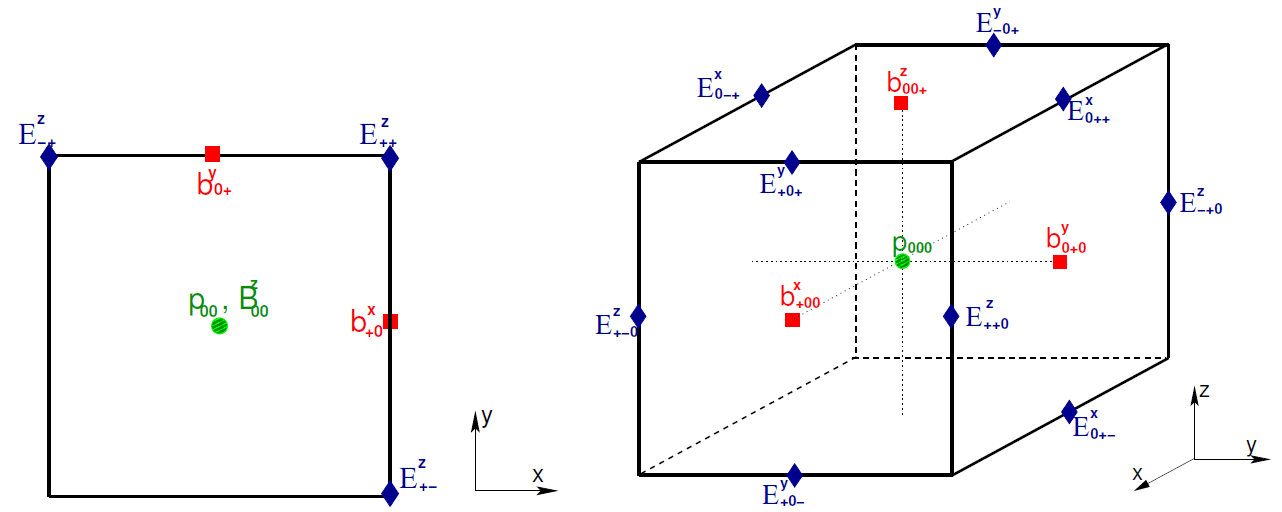
\includegraphics[width=0.8\linewidth]{images/ConstrainedTransports_img1.png}
    \caption{Localización de los puntos en las celdas de 2 y 3 dimensiones. Las componentes del campo magnético se encuentran en las caras, mientras que aquellas del campo eléctrico se posicionan en las aristas.}
    \label{fig:ConstrainedTranspor_1}
\end{figure}
Estos valores escalonados del campo magnético se obtienen como un promedio ponderado por el área, y se actualizan con el teorema de Stokes de la siguiente manera:
\begin{align*}
    \int \left( \frac{\partial \mathbf{B^{(s)}}}{\partial t} + \mathbf{\nabla \times E} \right) \cdot d\mathbf{S_d} = 0
\end{align*}
Con $\mathbf{E}$ el campo eléctrico, cuyas componentes se encuentran en las aristas de las celdas y son calculadas por reconstrucción o promediado, dependiendo del método especificado.

\medskip

El método pertinente es el aritmético, como se observa en la definición \lstinline[language=C]{CT_EMF_AVERAGE = ARITHMETIC}. En este, se realiza un simple promedio aritmético de los flujos calculados.

\medskip

El método de transporte constreñido asegura una condición solenoidal mantenida al grado de precisión de la máquina mientras se inicialice el campo utilizando un potencial vectorial, el cual es el caso presente en vista de \lstinline[language=C]{ASSIGN_VECTOR_POTENTIAL = YES}, siendo entonces el campo magnético:
\begin{subequations}\label{eq:BField_Vectorpotential}
    \begin{align}
        B_r &= \frac{1}{r \sin \theta} \frac{\partial (\sin \theta A_\phi)}{\partial \theta} \\[5pt]
        B_\theta &= -\frac{1}{r} \frac{\partial (r A_\phi)}{\partial r}
    \end{align}
\end{subequations}

\subsection{Condiciones de frontera}

Observando el bloque de condiciones de frontera dentro del archivo \lstinline[language=C]{pluto_03.ini}.
\begin{lstlisting}[language=C, caption={Definiciones de condiciones de frontera (pluto\_03.init)}, label={lst:ini_boundary}]
[Boundary]

X1-beg        userdef
X1-end        outflow
X2-beg        axisymmetric
X2-end        axisymmetric
X3-beg        outflow
X3-end        outflow
\end{lstlisting}

\subsubsection{\texorpdfstring{Frontera angular ($1 \leq r \leq 20$)}
  {Frontera angular (1 <= r <= 20)}}

La condición \lstinline[language=C]{userdef} para la frontera interna de $r$ (\lstinline[language=C]{X1_BEG}) establece el uso de la función \lstinline[language=C]{UserDefBoundary} dentro del archivo \lstinline[language=C]{init.c} de la manera descrita en Cód.\ref{lst:userdefboundary}.
\begin{lstlisting}[language=C, caption={Definición de condición en la frontera radial interna.}, label={lst:userdefboundary}]
void UserDefBoundary (const Data *d, RBox *box, int side, Grid *grid) 
/*! 
 *  Assign user-defined boundary conditions.
 *  At the inner boundary we use outflow conditions, except for
 *  velocity which we reset to zero when there's an inflow
 *
 *********************************************************************** */
{
  int     i, j, k, nv;
  double  *x1, *x2, *x3;
  static double vR1[NVAR];
  double R;

  x1 = grid->x[IDIR];
  x2 = grid->x[JDIR];
  x3 = grid->x[KDIR];
 
  if (side == X1_BEG){
    if (box->vpos == CENTER){
      BOX_LOOP(box,k,j,i){
        for (nv = 0; nv < NVAR; nv++){
          d->Vc[nv][k][j][i] = d->Vc[nv][k][j][IBEG];
        }
        d->Vc[VX1][k][j][i] = MIN(d->Vc[VX1][k][j][i],0.0); 
      }
    }else if (box->vpos == X2FACE){
      #ifdef STAGGERED_MHD
//       BOX_LOOP(box,k,j,i) d->Vs[BX2s][k][j][i] = d->Vs[BX2s][k][j][IBEG];
      #endif
    }
  }
}

\end{lstlisting}
En este caso, la frontera radial interna puede representar la superficie o vecindad del objeto central masivo que atrae al toroide. El código Cód.\ref{lst:userdefboundary} define una condición de salida libre (\textit{outflow}), copiando el valor de la primera celda activa hacia las celdas exteriores de la frontera ---visto en \lstinline[language=C]{d->Vc[nv][k][j][i] = d->Vc[nv][k][j][IBEG]}--- generando un gradiente nulo y permitiendo que las propiedades del plasma fluyan hacia afuera sin resistencia. Adicionalmente, \lstinline[language=C]{d->Vc[VX1][k][j][i] = MIN(d->Vc[VX1][k][j][i],0.0)} fuerza que la velocidad en la frontera radial sea siempre negativa o cero, de forma que el material del toroide caida hacia el objeto central y prohibiendo que material entre desde la frontera fantasma hacia el dominio de trabajo (esto evita la inyección espuria de masa desde el origen).

\medskip

Adicionalmente es posible observar el condicional \lstinline[language=C]{else if (box->vpos == X2FACE)}, dentro del cual se relega el manejo y actualización del gradiente normal del campo magnético al esquema CT anterior.

\medskip

La condición \lstinline[language=C]{outflow} en la frontera externa de $r$ establece un gradiente nulo, $\partial q / \partial n = 0$ para q, $\mathbf{v}$ y $\mathbf{B}$. Esto implica una condición de Neumann de orden cero con pendiente nula en el borde, cuya forma en la última celda activa $N$ es:
\begin{align*}
    q_{N + k} = q_N \quad k = 1, \ldots, n_g 
\end{align*}
Esto implica que el plasma fluye hacia el exterior del dominio de trabajo sin experimentar cambios drásticos, evitando relfexiones espurias.

\subsubsection{\texorpdfstring{Frontera angular ($0 \leq \theta \leq \pi$)}
  {Frontera angular (0 <= theta <= pi)}}

La condición \lstinline[language=C]{axisymmetric} para las fronteras de $\theta$ establece paredes rígidas, en las cuales las componentes normales y angulares cambian de signo:
\begin{align*}
    q \to q, 
    \quad 
    \left\{\begin{array}{c}
        v_n \to -v_n \\
        B_n \to -B_n
    \end{array}\right. , 
    \quad 
    \left\{\begin{array}{c}
        v_\phi \to -v_\phi \\
        B_\phi \to -B_\phi
    \end{array}\right. ,
    \quad 
    \left\{\begin{array}{c}
        v_{axis} \to v_{axis} \\
        B_{axis} \to B_{axis}
    \end{array}\right.
\end{align*}
Siendo $axis$ la dirección paralela al eje de simetría de las coordenadas ($r$, $\theta$ = 0). Así, la cuarta condición establece que las componentes de velocidad y campo magnético paralelas al eje radial se copian de forma simétrica, mientras que las angulares invierten signo.

\subsection{Estado del arte}

Papaloizou y Pringe\cite{Papaloizou} estudiaron en 1984 la estabilidad dinámica de toros con un momento angular específico constante (rotación prescrita), mostrando que son inestables en modos azimutales de bajo orden que evolucionan dentro de escalas de tiempo dinámicas. Este comportamiento se denominó \textit{inestabilidad de Papaloizou-Pringle} (PP) y posteriormente se atribuyó a las interacciones entre ondas en los bordes interno y externo del toro (Goldreich y Goodman, 1986)\cite{Goldreich}.

\medskip

Hawley (2000)\cite{Hawley} estudia un número de simulaciones magnetohidrodinámicas globales y tridimensionales de toros con un campo magnético poloidad ($B_\theta$) débil, encontrando que la inestabilidad magnetorrotacional (MRI estudiada en 1991 por Balbus y Hawley)\cite{HawleyMRI} produce turbulencia y transporte exterior de momento angular, permitiendo la acreción. Permite definir la configuración del toro a partir del potencial vector $A_\phi = B_0(\rho - \rho_{\rm cut})$ y $\beta$ alto.

\medskip

Kuwabara, Shibata, Kudoh y Matsumoto (2005)\cite{Kuwabara} realizaron estudios pertinentes al mecanismo de aceleración de jets magnetohidrodinámicos resistivos por medio de simulaciones axisimétricas en sistemas MHD no lineales. Describen la ecuación de equilibrio del toro para el caso de momento angular constante ($a = 0$) presentada en la Eq.\ref{eq:equilibrium}. 

\medskip

Estos trabajos ofrecen avances fundamentales para el desarrollo de este trabajo, describiendo el comportamiento del toro en las condiciones adecuadas y determinando los campos de estudio por fuera del alcance del mismo. Papaloizou y Pringe introducen la idea de una inestabilidad en modos azimutales de momento angular constante, caso no estudiado durante el desarrollo principal del presente informe. Hawley establece la existencia de una inestabilidad adicional relacionada al campo magnético mientras que Kuwabara y compañía presentan el equilibrio en dos dimensiones.

\section{Metodología}

Para realizar el debido proceso de comparación, se ejecuta en primera instancia el código de PLUTO, utilizando como se ha mencionado anteriormente, los parámetros de \lstinline[language=C]|definitions_03.h| y \lstinline[language=C]|pluto_03.ini|. La única diferencia se encuentra en la alteración de los límites temporales, los cuales se aumentaron para visibilizar un mayor rango de evolución dentro del sistema.

\medskip

Con esto se obtiene un conjunto de archivos \lstinline[language=C]|.dbl| en cada paso de tiempo, con las variables $prs$, $rho$, $vx1$, $vx2$, $vx3$, $Bx1$, $Bx2$, $Bx3$ y $tr1$ en la malla bidimensional definida. Utilizando el paquete \lstinline[language=C]|pyPLUTO| es posible graficar estas variables para una posterior comparación.

\medskip

Una vez conseguidos los resultados de la simulación se realiza un intento de reproducción de los resultados en Python. Este procedimiento se divide en: creación de malla, inicialización, condiciones de frontera y solución temporal. Estos pasos se realizan siguiendo la estructura general del procedimiento descrito por el código PLUTO en \lstinline[language=C]|init.c| y otros.

\section{Simulación PLUTO}

Utilizando las configuraciones definidas en los archivos \lstinline[language=C]{definitions_03.h} y \lstinline[language=C]{pluto_03.ini} es posible obtener los gráficos para el comportamiento espacial de las variables de interés; $\rho$, $v_r$, $v_\theta$, $B_r$, $B_\theta$ y $p_t$ presentados en la Fig.\ref{fig:step_0000_PLUTO}. 
\begin{figure}[H]
  \centering
  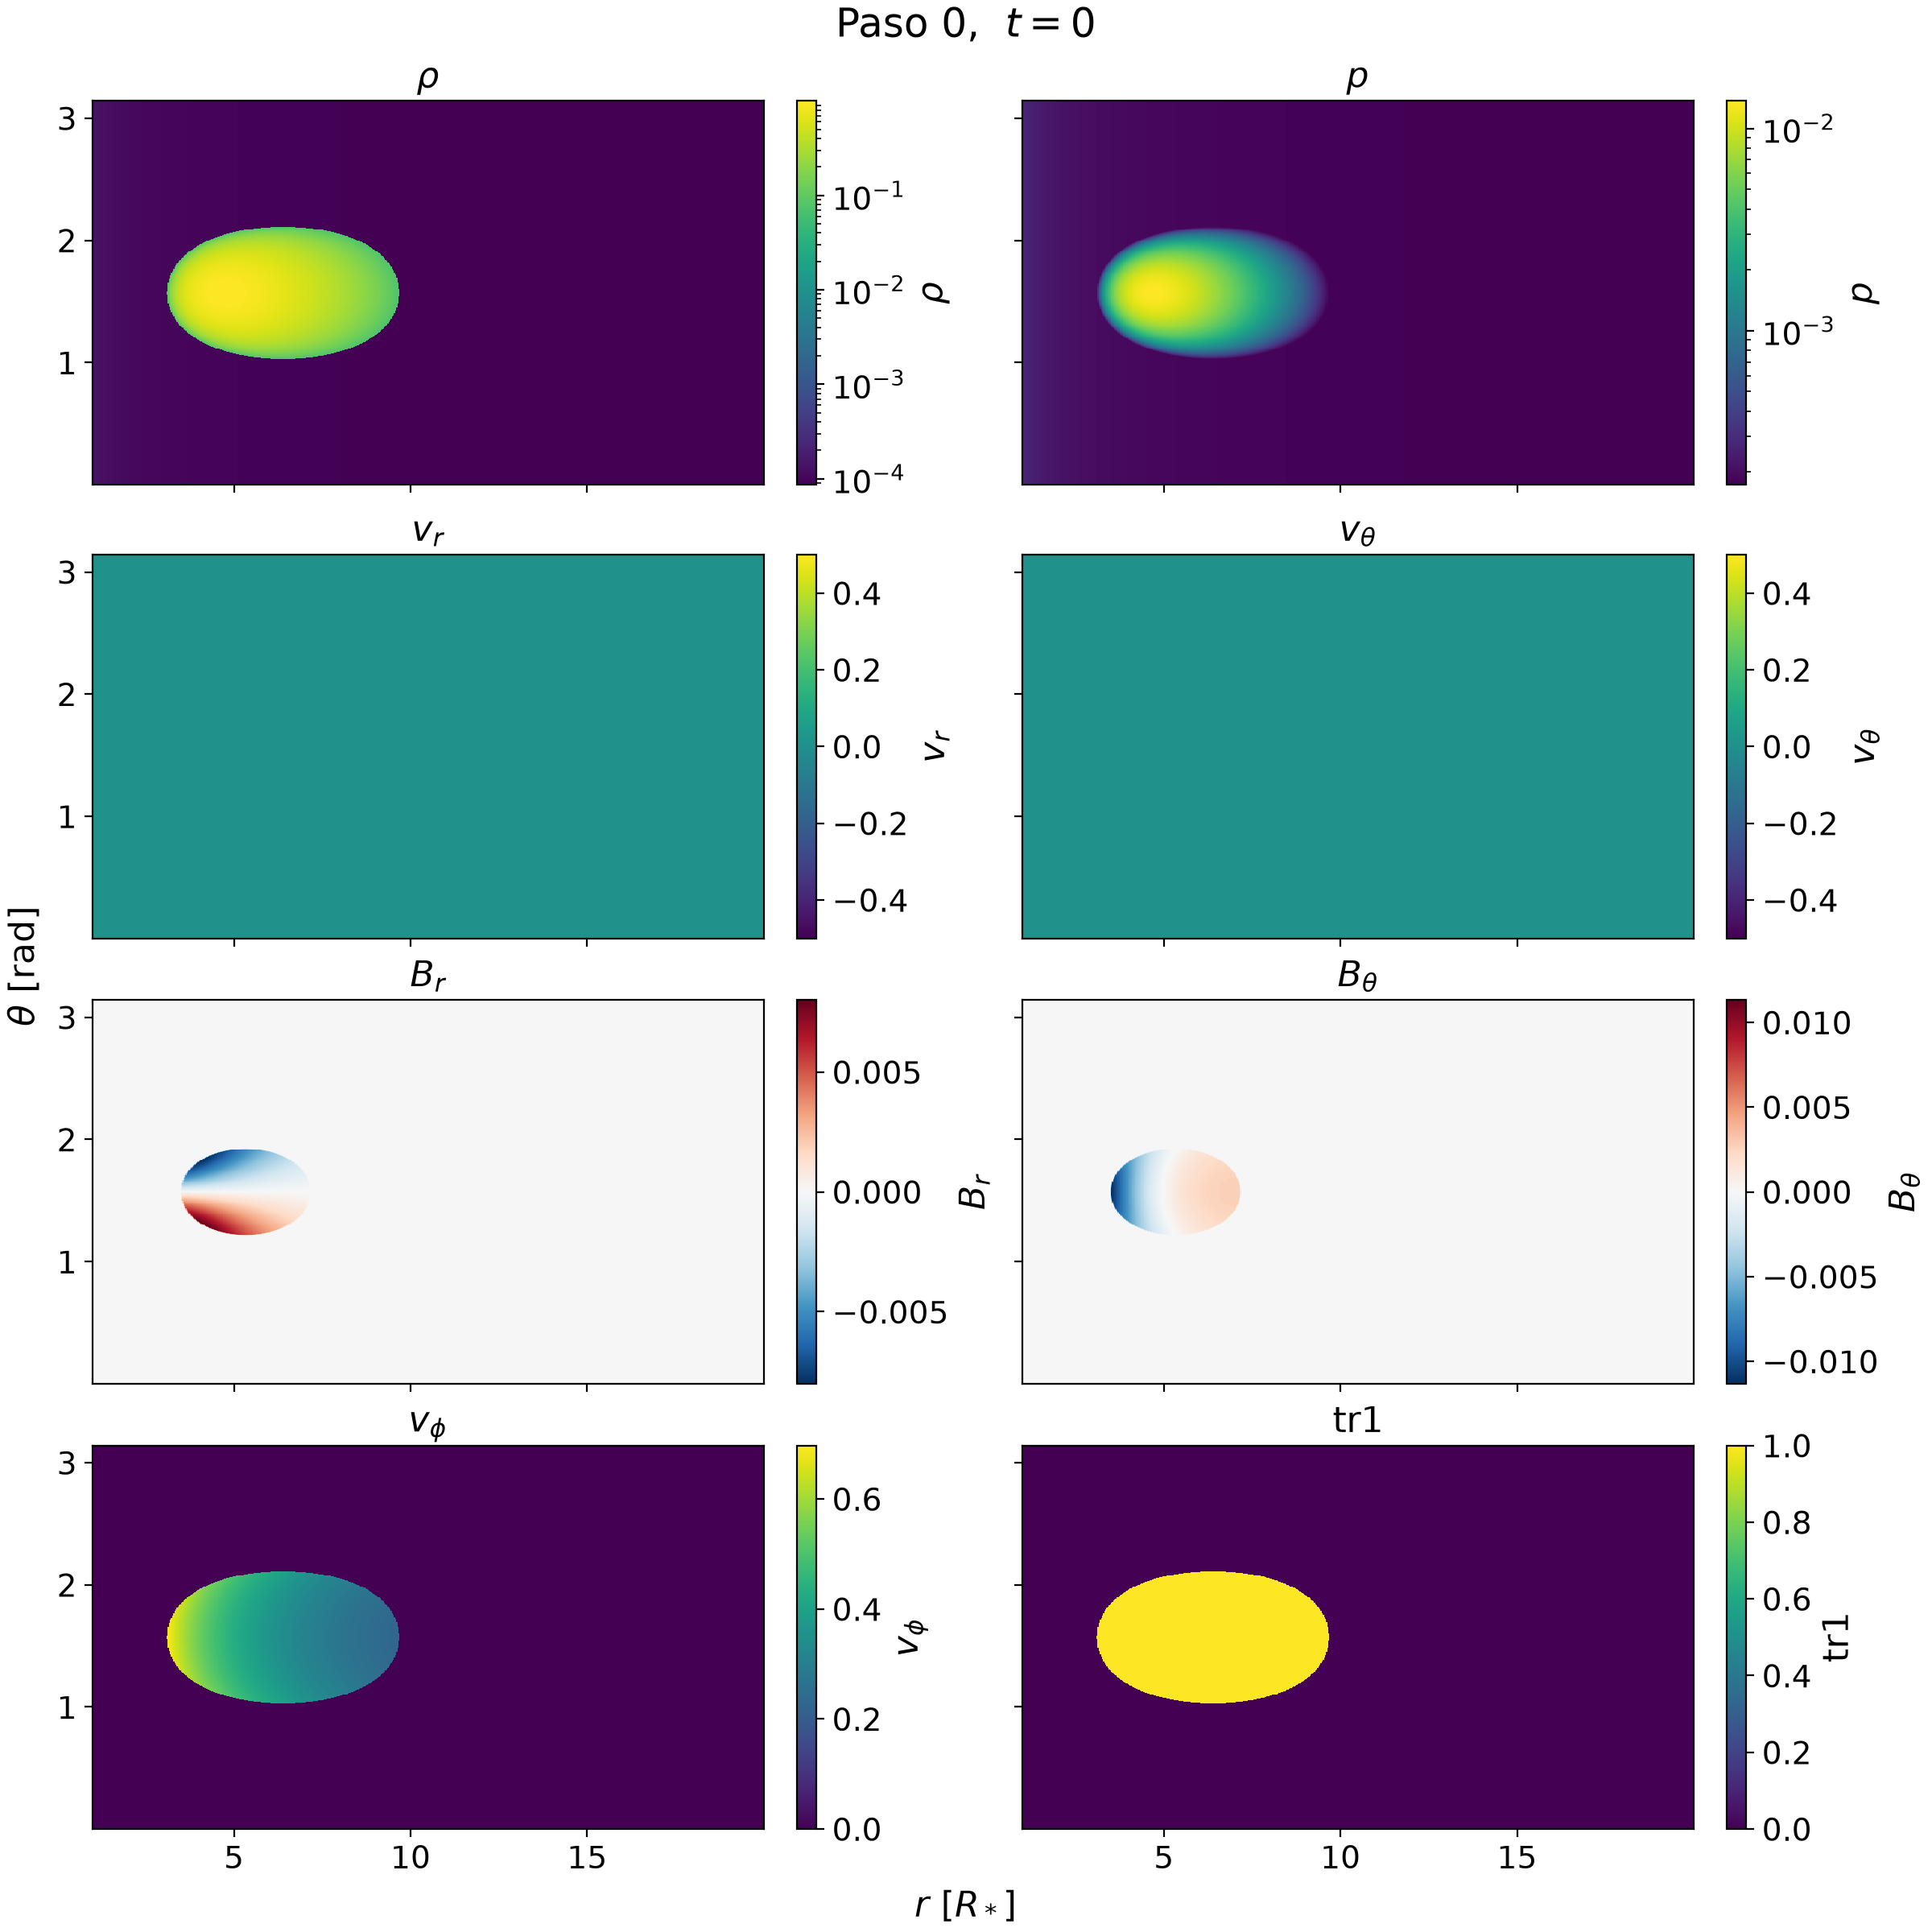
\includegraphics[width=\textwidth]{images/step_0000/panel.png}
  \caption{Estado inicial del toro ($t=0$), calculado por PLUTO.}
  \label{fig:step_0000_PLUTO}
\end{figure}
Para esto se utilizaron las siguientes configuraciones, guardadas en \lstinline[language=C]{pluto.ini}:
\begin{lstlisting}[language=C, caption={Parámetros de grilla, tiempo y solucionador para simulación del toro por PLUTO}, label={lst:pluto.ini}]
[Grid]

X1-grid   2   1.0  320 u   11.0                72  s 20.0
X2-grid   3   0.0   72 s   0.785398163397448  256  u 2.35619449019234   72  s  3.14159265358979
X3-grid   1   0.0    1 u   1.0

[Time]

CFL              0.4
CFL_max_var      1.1
tstop            5.0
first_dt         1.e-4

[Solver]

Solver         hlld

[Parameters]

RMIN                        3.0  
RMAX                        4.7  
RHO_CUT                     0.5  
BETA                        200.0  
ETA                         1.e-4  
SCALE_HEIGHT                2.0  
\end{lstlisting}
Según las definiciones del Cód.\ref{lst:pluto.ini}, la malla bidimensional se divide de la siguiente manera:
\begin{itemize}
    \item \textbf{Partición radial ($\mathbf{r}$)}: Dos segmentos globales. El primero de estos abarca el intervalo $r \in [1, 11]$ con 320 celdas uniformes (separación constante $\Delta r$). El segundo segmento, $r \in [11, 20]$ cuenta con 72 celdas estiradas (la separación aumenta conforme recorremos el segmento). En total se tienen 392 celdas activas radiales, comprendiendo el intervalo global $r \in [1, 20]$.
    \item \textbf{Partición angular ($\mathbf{\theta}$)}: Tres segmentos globales. El primero define el intervalo $\theta \in [0, \pi/4]$ con 72 celdas estiradas. El siguiente comprende $\theta \in [\pi/4, 3\pi/4]$ con 256 celdas uniformes. Finalmente el tercer segmentos abarca los valores $\theta \in [3\pi/4, \pi]$ con 72 celdas estiradas. En total se trabajan 400 celdas activas angulares, dentro del intervalo $\theta \in [0, \pi]$.
\end{itemize}
Respecto a los parámetros físicos del sistema, podemos observar que el toro está definido por sus radios interior $r_{\min} = 3$ y el radio de máxima densidad $r_{\max} = 4.7$. Adicionalmente tenemos la densidad de corte para el potencial vector $\rho_{\rm cut} = 0.5$, junto con el parámetro del plasma $\beta = 200$ y la razón entre densidades del toro y la atmósfera $\eta = 1\times10^{-4}$.  

\medskip

Con las ecuaciones del estado inicial se obtiene la distribución de densidad, observando que el toro tiene una forma elíptica en el plano $(r, \theta)$, extiéndose hacia alrededor de $r\approx10$. Siendo que la unidad de densidad es $\rho_{\max}$, $\rho = 1$ se obtiene a la distancia esperada de $4.7$, y la densidad atmosférica se mantiene estable alrededor de $\rho_a = 10^{-4}$, en concordancia con el valor de $\eta$.

\medskip

Además, las velocidades radial y angular se mantienen nulas en todo el dominio (aunque en estas imágenes el rango se ensancha de $-0.5$ a $0.5$), esto es lo esperado al haber definido un estado inicial sin movimiento poloidal. Sí hay, sin embargo, un desplazamiento toroidal como es posible observar en la variable $vx3 = v_{\phi}$, indicando una rotación mayor cerca al borde interior que en el exterior, mientras que la atmósfera se mantiene estacionaria.

\medskip

Los campos radial y angular $B_r$, $B_{\theta}$ están confinados a una región menor dentro del toro, debido a la densidad de corte $\rho_{\rm{cut}}$, mientras que el campo azimutal $B_{\phi}$ se encuentra en ceros debido a que el campo inicial nace únicamente de la componente toroidal del potencial vector $A_{\phi}$.

\section{Reproducción por Python}

Con el objetivo de reproducir los resultados de PLUTO a través del lenguaje de programación Python, se buscó realizar un seguimiento detallado de cada paso de solución encontrado en los archivos del código de PLUTO. Como se mencionó con anterioridad, se dividió el flujo de trabajo en varios pasos: creación de la malla, inicialización, condiciones de frontera y solución temporal.



\begin{thebibliography}{99}

\bibitem{plutomanual}
Mignone, A. et al. (2024). PLUTO: User's Guide. \url{https://plutocode.ph.unito.it/documentation.html}

\bibitem{Papaloizou}
Papaloizou, J.C.B. \& Pringle, J.E. (1984). The dynamical stability of differentially rotating discs with constant specific angular momentum. \textit{Monthly Notices of the Royal Astronomical Society}. Vol. 208. \doi{10.1093/mnras/208.4.721}

\bibitem{Goldreich}
Goldreich, P. \& Goodman, J. (1986). The stability of accretion tori. \textit{Monthly Notices of the Royal Astronomical Society}. Vol. 221. \doi{https://doi.org/10.1093/mnras/221.2.339}

\bibitem{Hawley}
Hawley, J.F. (2000). Global Magnetohydrodynamical Simulations of Accretion Tori. \textit{The Astrophysical Journal}. Vol. 528. \doi{10.1086/308180}

\bibitem{HawleyMRI}
Hawley, J.F. \& Balbus, S.A. (1991). A Powerful Local Shear Instability in Weakly Magnetized Disks. \textit{Astrophysical Journal}. Vol. 376. \doi{10.1086/170270}

\bibitem{Kuwabara}
Kuwabara, T., Shibata, K., Kudoh, T. \& Matsumoto, R. (2005). The Acceleration Mechanism of Resistive Magnetohydrodynamic Jets Launched from Accretion Disks. \textit{Astrophysical Journal}. Vol. 621. \doi{https://doi.org/10.1086/427720}

\end{thebibliography}

\end{document}
